\documentclass[a4paper,11pt]{jsarticle}

% 数式
\usepackage{amsmath,amsfonts}
\usepackage{bm}
% 画像
\usepackage[dvipdfmx]{graphicx}
% bibTeX
\usepackage[backend = biber,style =apa, sorting =none,]{biblatex}

% 参考文献ファイルのリスト
% \addbibresource{references.bib}

% 等式番号を章ごとに割り振る
\makeatletter
\@addtoreset{equation}{section}
\def\theequation{\thesection.\arabic{equation}}
\makeatother

% listings(ソースコード)
\usepackage{listings}

\lstset{
basicstyle={\ttfamily},
identifierstyle={\small}
commentstyle={\smallitshape},
keywordstyle={\small\bfseries},
ndkeywordstyle={\small},
stringstyle={\small\ttfamily},
frame={tb},
breaklines=true,
columns=[l]{fullflexible},
numbers=left,
xrightmargin=0zw,
xleftmargin=3zw,
numberstyle={\scriptsize},
stepnumber=1,
numbersep=1zw,
lineskip=-0.5ex
}
\renewcommand{\lstlistingname}{}

\begin{document}

\title{計算機科学実験4 音声 レポート1}
\author{安済翔真}
\date{\today}
\maketitle

\tableofcontents
\newpage

\section{機能・プログラム説明}

課題1では音声の基本的な情報を表示するプログラムを作成した。
この章では作成した具体的な機能について説明する。
画面全体は図\ref{fig:work2_app}のようになっている。下のVoice ChangeやTremoloの部分は
課題2の機能のため、レポートでは説明しない。

\begin{figure}[h]
\centering
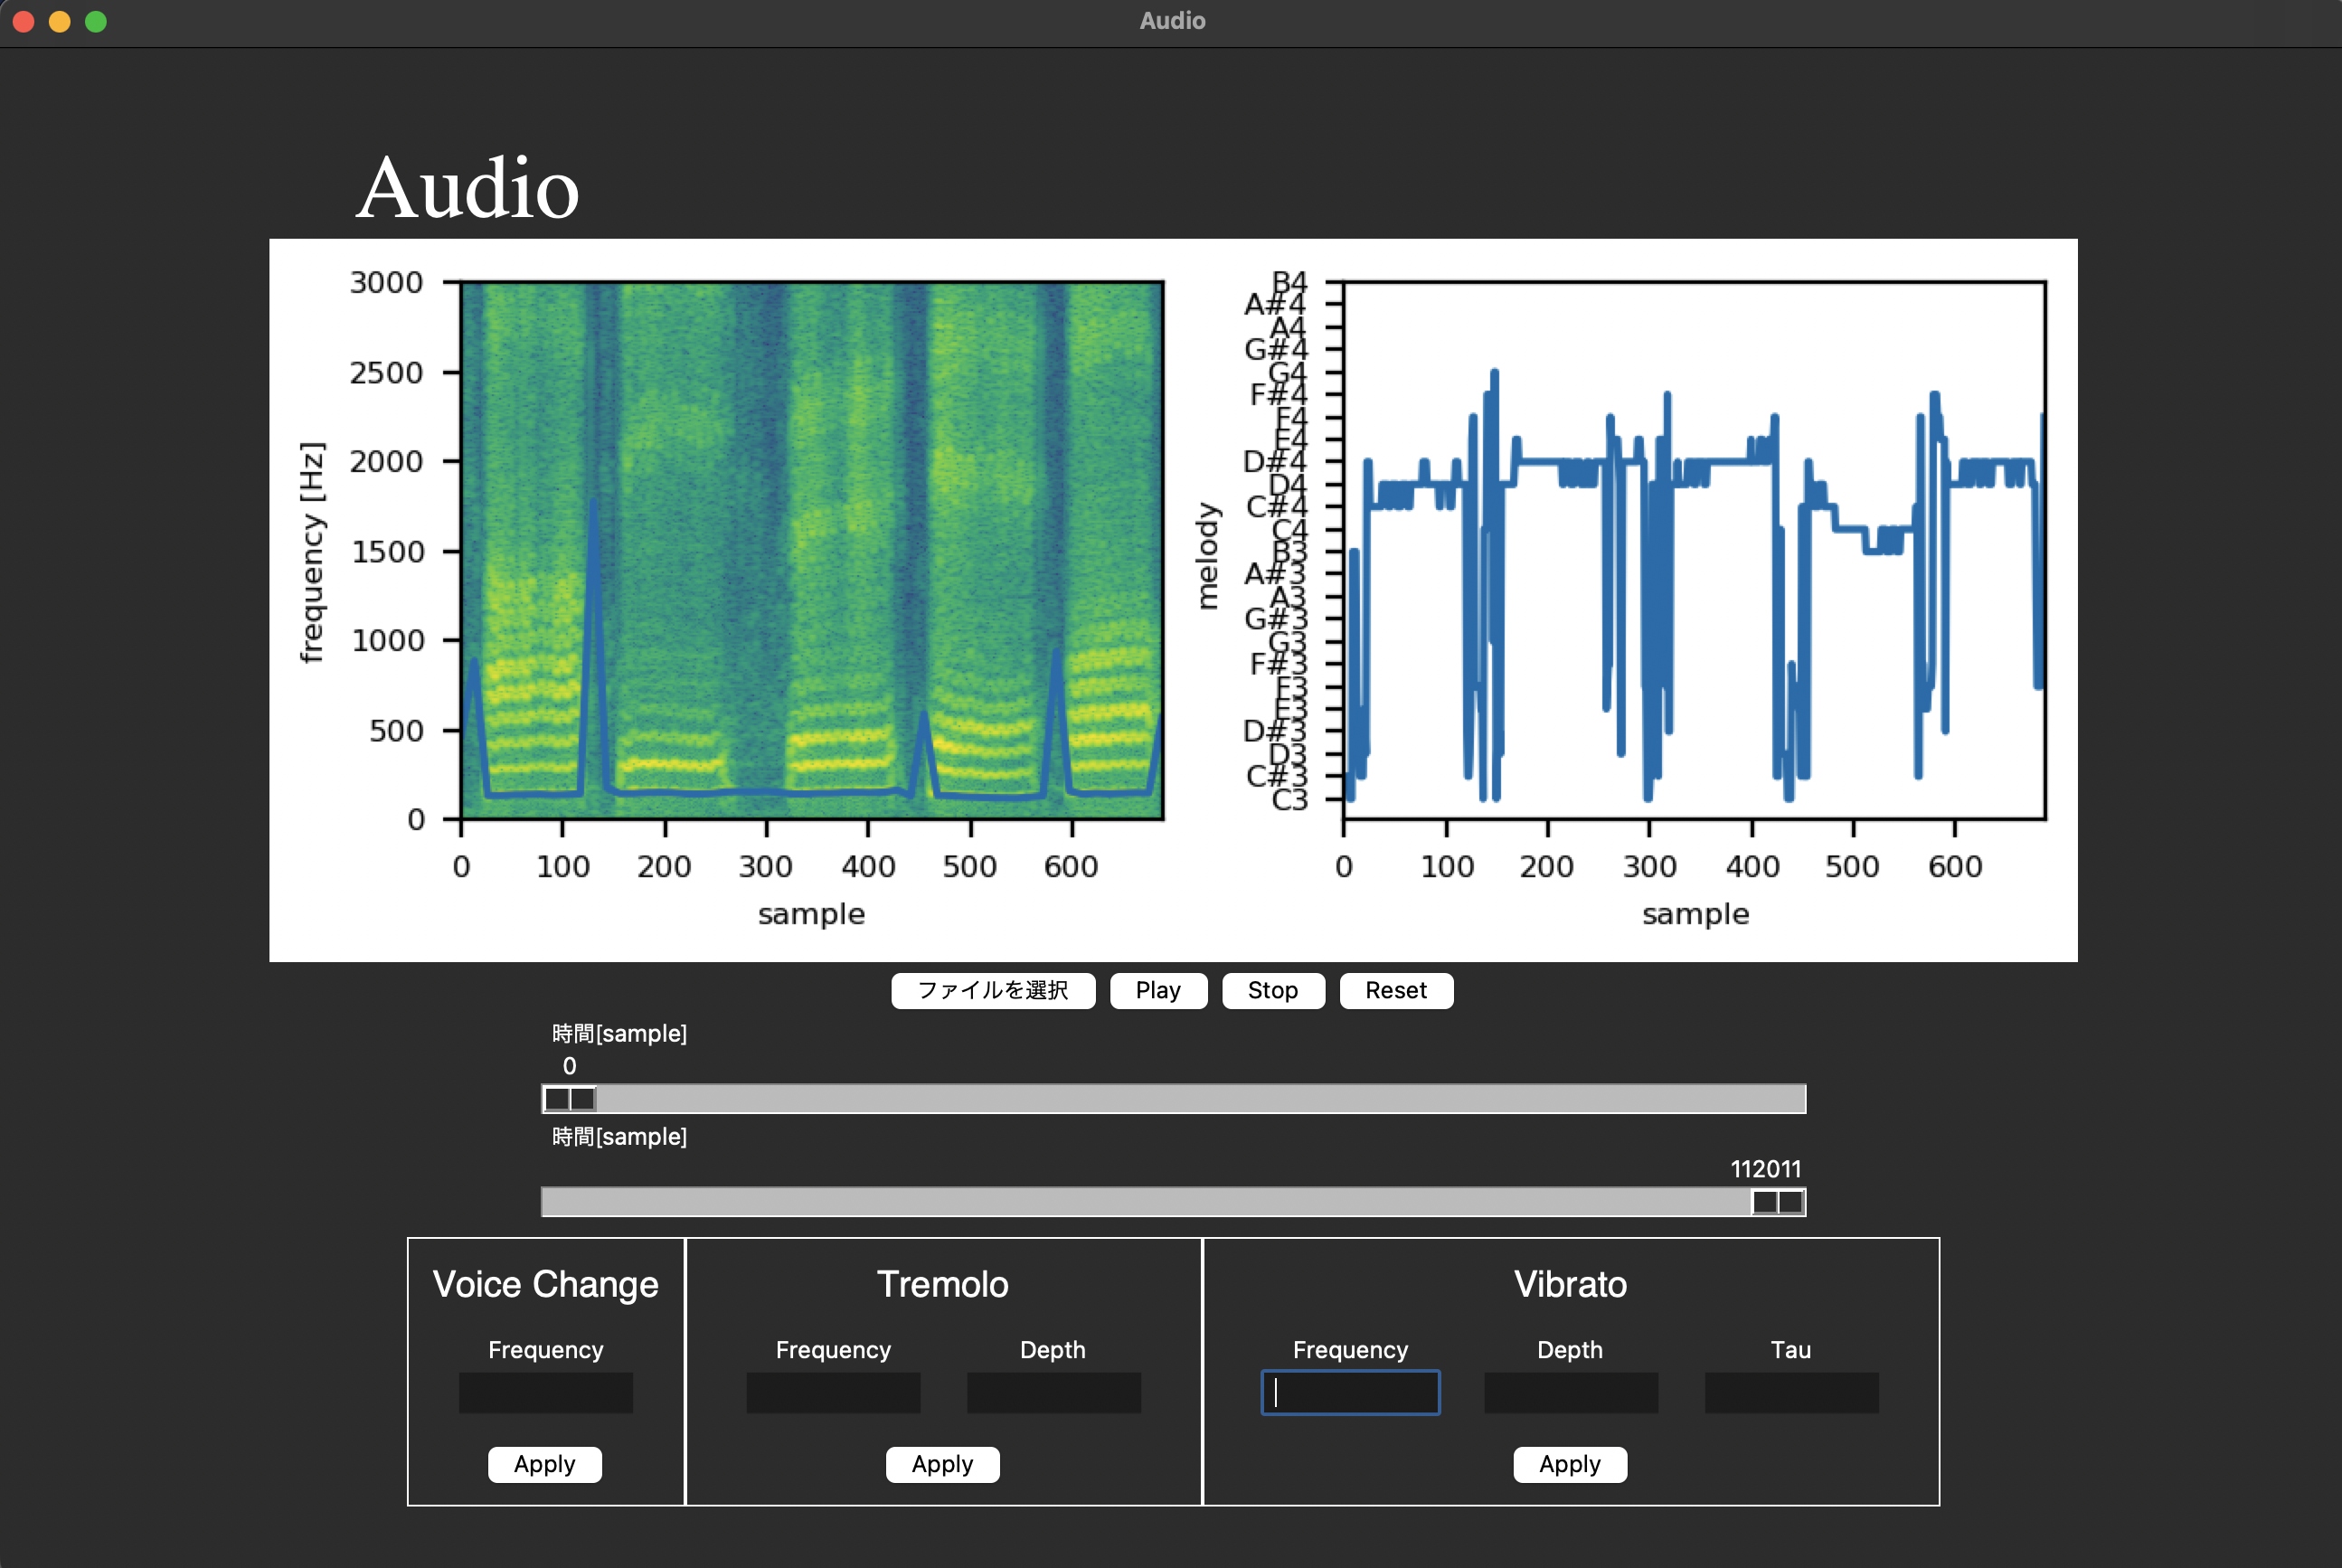
\includegraphics[keepaspectratio, width=13cm]
{./images/work2_app.png}
\caption{画面全体}
\label{fig:work2_app}
\end{figure}

\subsection{ファイル選択}
ファイル選択機能を実装した。ファイル選択ボタン(図\ref{fig:select_file})を押すと、ファイル選択ダイアログが表示される。
選択したファイルを読み取り、表示対象の音声データとして扱う。

\begin{figure}[h]
\centering
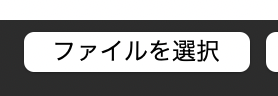
\includegraphics[keepaspectratio, scale = 1.0]
{./images/select_file.png}
\caption{ファイル選択ボタン}
\label{fig:select_file}
\end{figure}

ファイル読み取りのプログラムはコード\ref{code:load_file1}, \ref{code:load_file2}の通りである。
コード\ref{code:load_file1}はtkinterのfiledialogを用いてファイル選択ダイアログを表示し、
選択したファイル名を取得する。コード\ref{code:load_file2}はlibrosaを用いて音声データを読み取る。

\begin{lstlisting}[caption=ファイル読み取り1,label=code:load_file1]
  filename = tk.filedialog.askopenfilename()
  self._c.load_file(filename)
\end{lstlisting}

\begin{lstlisting}[caption=ファイル読み取り2,label=code:load_file2]
def load_waveform(filename):
  x, _ = librosa.load(filename, sr=SR)
  return x
\end{lstlisting}

\subsection{スペクトログラムの表示}
選択したファイルの音声のスペクトログラムを表示する機能を実装した。
コード\ref{code:calc_spectrogram}はスペクトログラムを計算するプログラムである。
numpyのhamming関数を用いて窓掛けを行い、FFTを行う。
その後、対数振幅スペクトルを計算し、配列に保存する。

\begin{lstlisting}[caption=スペクトログラム計算,label=code:calc_spectrogram]
def spectrogram(waveform, size_frame, size_shift):
  spectrogram = []
  hamming_window = np.hamming(size_frame)

  for i in np.arange(0, len(waveform) - size_frame, size_shift):
    idx = int(i)
    x_frame = waveform[idx: idx + size_frame]

    # 窓掛けしたデータをFFT
    fft_spec = np.fft.rfft(x_frame * hamming_window)

    # 振幅スペクトルを対数化
    fft_log_abs_spec = np.log(np.abs(fft_spec))

    # 配列に保存
    spectrogram.append(fft_log_abs_spec)
  return spectrogram
\end{lstlisting}

コード\ref{code:show_spectrogram}はスペクトログラムを表示するプログラムである。
matplotlibのimshow関数を用いてスペクトログラムを表示する。
\begin{lstlisting}[caption=スペクトログラム表示,label=code:show_spectrogram]
self.__ax.imshow(
    np.flipud(np.array(spectrogram).T),
    extent=[0, len(spectrogram), 0, SR / 2],
    aspect='auto',
    interpolation='nearest',
)
self.__ax.set_ylim(0, 3000)
\end{lstlisting}

\subsection{基本周波数の表示}
選択したファイルの音声の基本周波数を表示する機能を実装した。
コード\ref{code:calc_f0}は基本周波数を計算するプログラムである。
まず、numpyのcorrelate関数を用いて自己相関係数を計算する。
その後、ピークを検出し、ピークのインデックスを取得する。
最後に、ピークのインデックスから基本周波数を計算する。

\begin{lstlisting}[caption=基本周波数計算,label=code:calc_f0]
def get_f0(waveform, sampling_rate):
  autocorr = np.correlate(waveform, waveform, 'full')
  autocorr = autocorr[len(autocorr) // 2:]  # 不要な前半を捨てる

  # ピークを検出
  peak_indices = [i for i in range(len(autocorr)) if is_peak(autocorr, i)]
  peak_indices = [i for i in peak_indices if i != 0]  # 最初のピークは除く

  if len(peak_indices) == 0:
    return 0

  max_peak_index = max(peak_indices, key=lambda index: autocorr[index])

  # 基本周波数を推定
  f0 = sampling_rate / max_peak_index
  return f0
\end{lstlisting}

コード\ref{code:show_f0}は基本周波数を表示するプログラムである。
matplotlibのplot関数を用いて基本周波数を表示する。
スペクトログラムと同じx軸を用いるため、x軸のデータはスペクトログラムのデータを用いる。

\begin{lstlisting}[caption=基本周波数表示,label=code:show_f0]
  x_data = np.linspace(0, len(spectrogram), len(f0s))
  self.__ax.plot(x_data, f0s)
\end{lstlisting}

\subsection{音程の表示}
選択したファイルの音声の音程を表示する機能を実装した。
コード\ref{code:calc_pitch}は音程を計算するプログラムである。
nn2hz関数はMIDIノートナンバーを周波数に変換する関数である。
shs関数はスペクトルを用いて音程を計算する関数である。
候補の音程(NOTES)の各周波数について、スペクトルの対数振幅スペクトルを用いて尤度を計算する。
尤度を計算する際は、対象の音程の「倍音」の強さも考慮した。特に、倍音の強さは
0.8の指数関数的な減衰を考慮することで精度が大幅に向上した。

\begin{lstlisting}[caption=音程計算,label=code:calc_pitch]
def nn2hz(nn):
  return 440.0 * 2 ** ((nn - 69) / 12.0)

def shs(spectrum, sample_rate, size_frame):
  likelihood = np.zeros(len(NOTES))
  for i in range(len(likelihood)):
    base_freq = nn2hz(NOTES[i])
    for j in range(1, 16):
      freq = base_freq * j
      fft_idx = int(freq * size_frame / sample_rate)
      likelihood[i] += 0.8**j * np.exp(spectrum[fft_idx])
  return NOTES[np.argmax(likelihood)]

\end{lstlisting}

コード\ref{code:show_pitch}は音程を表示するプログラムである。
matplotlibのplot関数を用いて音程を表示する。
yticksでy軸のラベルを設定している。ラベルの内容はC3からB4までの音程を表示することで、
表示される音程がわかりやすくなるようにした。

\begin{lstlisting}[caption=音程表示,label=code:show_pitch]
  plt.plot(list(map(lambda x: x - NOTES[0], melody)))
  plt.yticks(np.arange(24),
         list(["C3", "C#3", "D3", "D#3", "E3", "F3", "F#3", "G3",
               "G#3", "A3", "A#3", "B3", "C4", "C#4", "D4", "D#4",
               "E4", "F4", "F#4", "G4", "G#4", "A4", "A#4", "B4"])
         )
\end{lstlisting}

\subsection{音声の再生・停止}

選択したファイルの音声を再生・停止する機能を実装した。
コード\ref{code:play}は音声を再生するプログラムである。
既に音声が再生中の場合は、一旦再生を停止してから再度再生をすることで、
同じ音声を連続して再生することができる。

\begin{lstlisting}[caption=音声再生,label=code:play]
  if self.__play_obj is not None:
    self.__play_obj.stop()
  self.__play_obj = self.__wave_obj.play()
\end{lstlisting}

コード\ref{code:stop}は音声を停止するプログラムである。
音声が再生中の場合のみ、音声を停止する。

\begin{lstlisting}[caption=音声停止,label=code:stop]
  if self.__play_obj is None:
    return
  self.__play_obj.stop()
  self.__play_obj = None

\end{lstlisting}

\subsection{表示区間・再生区間の限定}

スペクトログラムや音程の表示、及び音声の再生区間を限定する機能を実装した。
コード\ref{code:limit}は表示区間・再生区間を限定するプログラムである。
startの値はendの値より大きくならないようバリデーションを行った。

\begin{lstlisting}[caption=表示区間・再生区間の限定,label=code:limit]
  def set_start(self, start: int):
    if start >= self.__end - self.MIN_SIZE:
      return
    self.__start = start

  def set_end(self, end: int):
    if end <= self.__start + self.MIN_SIZE:
      return
    self.__end = end
\end{lstlisting}

コード\ref{code:show_limit}は区間を限定するUIを表示するプログラムである。
tkinterのScaleを用いて、スライダーのUIを表示している。
このコードにより、図\ref{fig:sliders}のようなUIが表示される。

\begin{lstlisting}[caption=区間を限定するUI,label=code:show_limit]
  self.slider = tk.Scale(
    command=self.__command,
    master=self._frame,
    from_=from_,
    to=to,
    label=u'時間[sample]',
    orient=tk.HORIZONTAL,
    length=700,
    width=15,
  )
\end{lstlisting}

\begin{figure}[h]
\centering
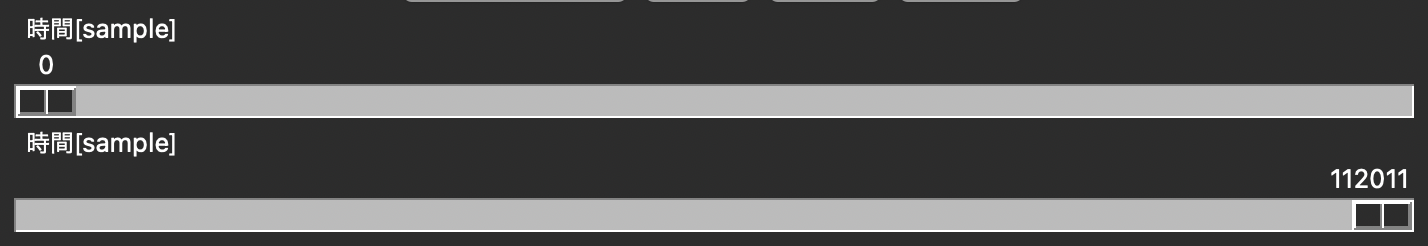
\includegraphics[keepaspectratio, width = 13cm]
{./images/sliders.png}
\caption{区間を限定するUI}
\label{fig:sliders}
\end{figure}

\section{実行例とテスト}
\subsection{ファイル選択}
ファイル選択ボタンを押すと、図\ref{fig:file_select_dialog}
のようなファイル選択ダイアログが表示される。
これにより、ファイル選択ボタンが正しく動作していることが確認できる。

\begin{figure}[h]
\centering
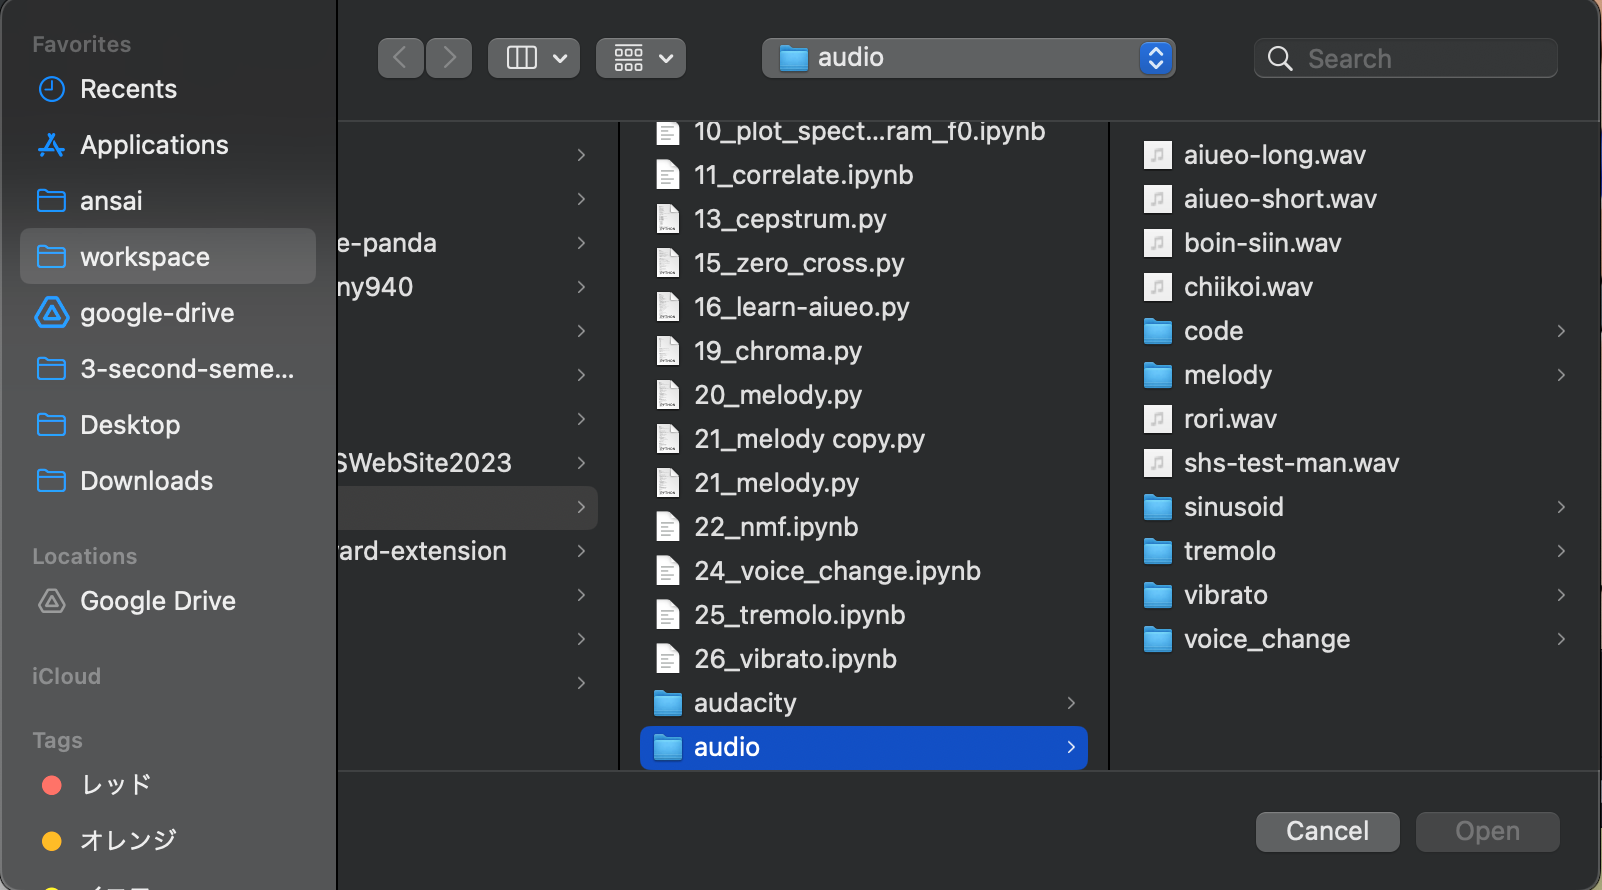
\includegraphics[keepaspectratio, width=13cm]
{./images/file_select_dialog.png}
\caption{ファイル選択ダイアログ}
\label{fig:file_select_dialog}
\end{figure}

\subsection{スペクトログラムの表示}

ファイルを選択すると、図\ref{fig:spectrogram}のようにスペクトログラムが表示される。
図\ref{fig:spectrogram}は「あいうえお」の音声のスペクトログラムである。
これにより、スペクトログラムが正しく表示されていることが確認できる。

\begin{figure}[h]
\centering
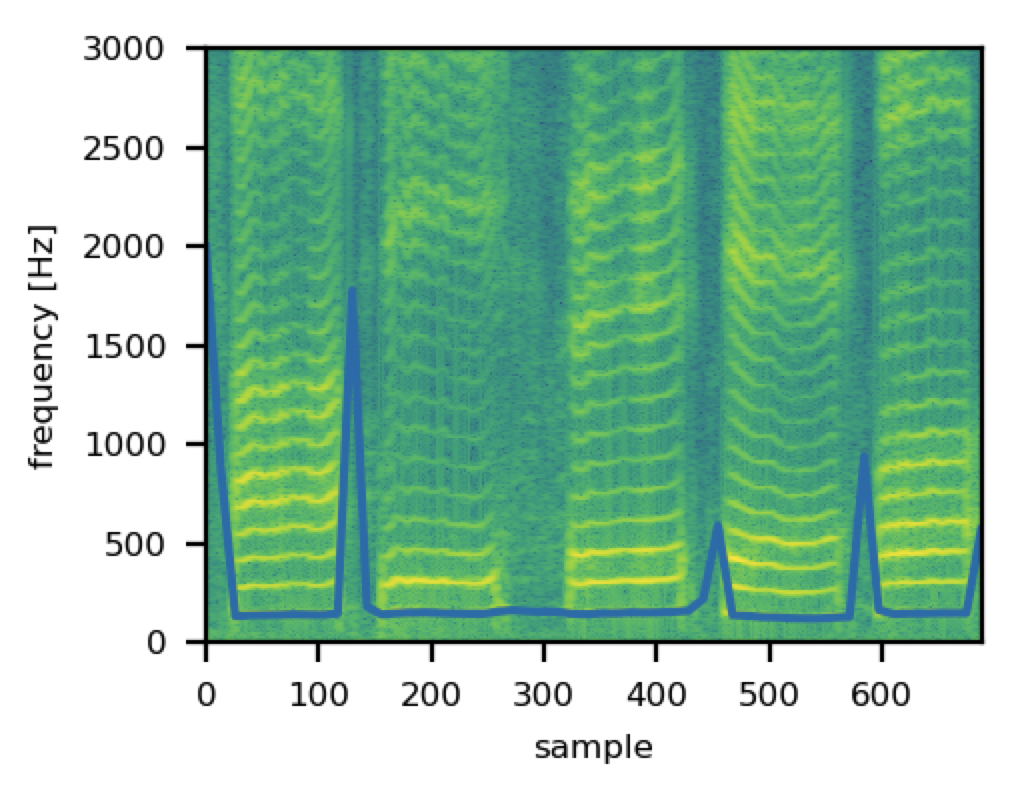
\includegraphics[keepaspectratio, width=13cm]
{./images/spectrogram.png}
\caption{スペクトログラム}
\label{fig:spectrogram}
\end{figure}

\subsection{基本周波数の表示}

ファイルを選択すると、図\ref{fig:f0}のように基本周波数が表示される。


\subsection{音程の表示}

\subsection{音声の再生・停止}

\subsection{表示区間・再生区間の限定}

\section{工夫点}
\subsection{ファイル選択機能}

\subsection{区間選択機能}
startの値がendの値より大きくならないようバリデーションを行った。

\subsection{音程の表示}

\subsection{音声の再生・停止機能}


\section{考察}

% \printbibliography[title=参考文献]

\end{document}
